\section{Informationstheorie}
\subsection{Typen von Datenquellen}
\subsubsection{Discrete Memoryless Source (DMS)}
\begin{itemize}
    \item Discrete heisst, dass die Quelle (zeitlich) einzelne Ereignisse liefert.
    \item Memoryless bedeutet, die Quelle erinnert sich beim Produzieren
    eines Ereignisses nicht an die Vorgeschichte.
    $\rightarrow$ Die Ereignisse sind (statistisch) unabhängig voneinander
\end{itemize}
\subsubsection{Binary Memoryless Source (BMS)}
\begin{itemize}
    \item Bei dieser Quelle handelt es sich um eine DMS, die aber nur zwei
    verschiedene Ereignisse erzeugt.
    \item Ausgabe ist eine Folge von 0 und 1
\end{itemize}
\subsection{Zweier-Logarithmus}
\begin{equation*}
    x = log_2(K) = \frac{log_{10}(K)}{log_{10}(2)}
\end{equation*}
\subsection{Gleiche Wahrscheinlichkeit}
\begin{itemize}
    \item Je mehr Fälle es gibt, desto seltener tritt ein bestimmtes Ereignis ein.
    \item Je seltener ein Ereignis ist, desto höher ist sein Informationsgehalt.
    \item $N$ sei wieder die Anzahl der möglichen Ereignisse. Wenn alle Ereigniswerte $x_n$ die Gleiche
    Auftretungswahrscheinlichkeit $P(x_n)$ haben, gilt:
    \begin{equation*}
        P(x_n) = \frac{1}{N} \rightarrow N = \frac{1}{P(x_n)}
    \end{equation*}
\end{itemize}
\subsection{Informationsgehalt von Ereignissen}
\begin{itemize}
    \item Je seltener ein Ereignis eintritt, desto grösser ist der
    Informationsgehalt (Überraschungseffekt)
    \item Die folgende Formel gilt allgemein:
    \begin{equation*}
        I(x_n) = log_2(\frac{1}{P(x_n)})
    \end{equation*}
\end{itemize}
\subsection{Entropie}
Den mittleren Informationsgehalt von Quellen nennt man Entropie:
\begin{equation*}
    H(X) = \sum_{n=0}^{N-1} P(x_n) \cdot log_2(\frac{1}{P(x_n)}) = \sum_{n=0}^{N-1} P(x_n) \cdot I(x_n)
\end{equation*}

Die Masseinheit der Entropie ist $Bit/Symbol$.
\subsubsection{Entropie Binary Memoryless Source}
Eine BMS kennt nur zwei Symbole. Ist $p$ die Auftretungswahrscheinlichkeit des eines Symbols, folgt dass $(1-p)$ jene des anderen Symbols ist.
\begin{equation*}
    H_b = p  \cdot log_2(\frac{1}{p}) + (1-p)  \cdot log_2(\frac{1}{1-p})
\end{equation*}
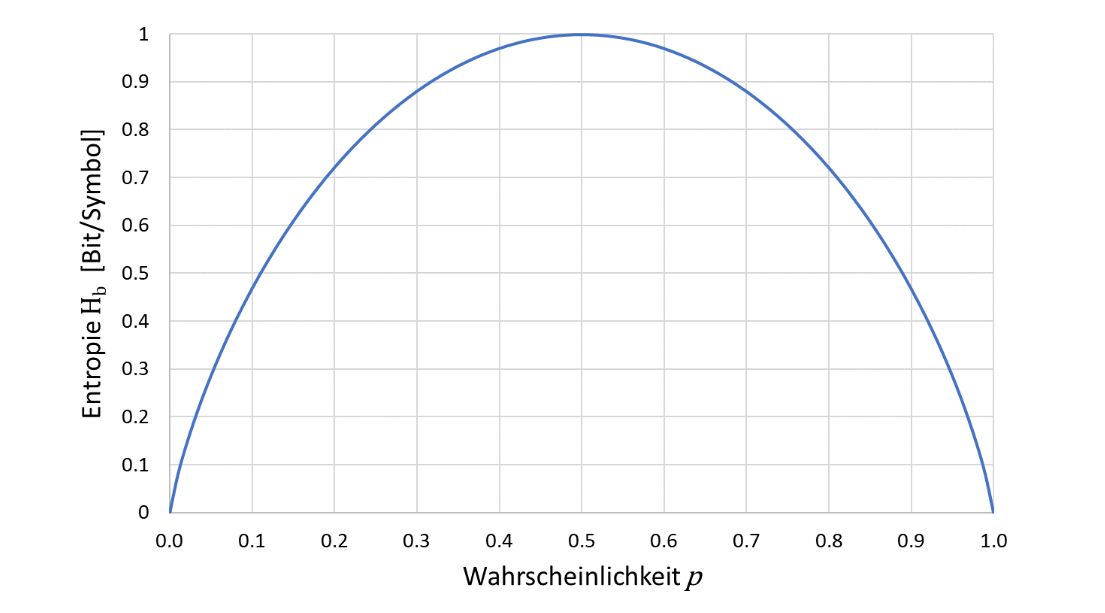
\includegraphics[scale=0.25]{binaere_Entropiefunktion}